\subsection{GUI}
Det vigtigste der skulle testes ved brugergrænsefladen var at den kunne sende en hvilken som helst kommando ved hjælp af SPI driveren. Dette blev testet ved at 
forbinde Analog Discovery til Devkit8000’s SPI ben. Derefter blev funktionen Logic Analyzer benyttet til at måle på outputtet. Det var vigtigt at vide hvornår 
kommandoen blev sendt ud. Da touchfunktionen ikke har været optimal på Devkit8000 blev funktion ”Planlæg åbning” brugt til at teste hvad outputtet fra Devkit8000
 var efter nedtællingen. Grunden til at funktionen ”Åbn nu” ikke blev brugt, var fordi at man skulle trykke mange gange på touchskærmen for at Devkittet ville 
 reagere. Dette bragte en uønsket usikkerhed i testen. Derfor var det mere hensigtsmæssigt at teste med funktionen ”Planlæg åbning da man her kan se hvornår 
 tiden udløber, og dermed hvornår der bør sendes en kommando ud. På figur \ref{PAA}, kan det ses hvordan, det var muligt at sende kommandoen 5 ved at bruge 
 ”Planlæg åbning” funktionen. 

\begin{figure}[H]
	\includegraphics[scale=1]{tex/Test/GUI-Test/Billeder/test_GUI}
	\caption{Åben nu funktionen implementerets}
	\label{PAA}
\end{figure}

\subsubsection{Test med virtuel klasse}
Der var problemer med modtagelse af kommandoer fra SPI. For at teste om GUI var korrekt implementeret, blev der lavet en virtuel klasse som fungerede som en 
stub. Denne klasse skulle simulere skrivning/læsning af data til/fra SPI device driveren. Istedet for at læse fra et SPI device i /dev, blev der læst fra en txt 
fil istedet. Da devices bliver behandlet som filer i Linux, ville funktionalitet i den virtuelle klasse ligge meget tæt på den egenlige implementering. Dermed 
kunne det testes om GUI kunne give status beskeder tilbage til brugeren, selvom SPI forbindelsen ikke var tilgængelig. På figur \ref{PAA} ses hvordan GUI meddeler 
bruger statusbeskeder på baggrund af den kommando som blev indlæst fra txt filen.

\begin{figure}[H]
	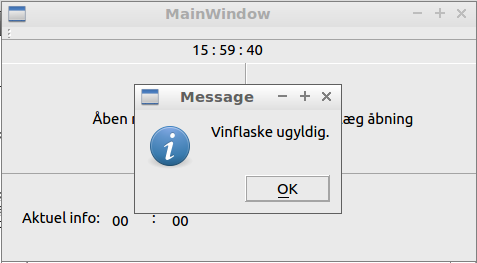
\includegraphics[scale=1]{tex/Test/GUI-Test/Billeder/Test_Virtuel_klasse_invalid}
	\caption{Test at virtuel klasse}
	\label{PAA}
\end{figure}